%% LyX 2.3.0 created this file.  For more info, see http://www.lyx.org/.
%% Do not edit unless you really know what you are doing.
\documentclass[english]{beamer}
\usepackage{lmodern}
\usepackage[T1]{fontenc}
\usepackage[latin9]{inputenc}
\usepackage{array}
\usepackage{rotating}
\usepackage{multirow}
\usepackage{footnote}
\usepackage{amsmath}
\usepackage{amssymb}
\usepackage{graphicx}

\makeatletter

%%%%%%%%%%%%%%%%%%%%%%%%%%%%%% LyX specific LaTeX commands.

\makesavenoteenv{tabular}

%% Because html converters don't know tabularnewline
\providecommand{\tabularnewline}{\\}

%%%%%%%%%%%%%%%%%%%%%%%%%%%%%% Textclass specific LaTeX commands.
% this default might be overridden by plain title style
\newcommand\makebeamertitle{\frame{\maketitle}}%
% (ERT) argument for the TOC
\AtBeginDocument{%
  \let\origtableofcontents=\tableofcontents
  \def\tableofcontents{\@ifnextchar[{\origtableofcontents}{\gobbletableofcontents}}
  \def\gobbletableofcontents#1{\origtableofcontents}
}

%%%%%%%%%%%%%%%%%%%%%%%%%%%%%% User specified LaTeX commands.
\usetheme{Warsaw}
% or ...

\setbeamercovered{transparent}
% or whatever (possibly just delete it)

\beamertemplatenavigationsymbolsempty

\renewcommand{\insertnavigation}[1]{}
\def\insertnavigation#1{\relax}

\titlegraphic{

\includegraphics[height=15mm]{fig/trimlogo} \hspace{10mm}

\includegraphics[height=15mm]{fig/uedinlogo} \hspace{10mm}

\includegraphics[height=15mm]{fig/eclogo}
}

\usepackage{multimedia}
%\usepackage{tikz}

\makeatother

\usepackage{babel}
\begin{document}

\title[3DRMS Challenge 2018]{3D Reconstruction Meets Semantics }

\subtitle{Reconstruction Challenge 2018}

\author[TrimBot2020]{Radim Tyle{\v c}ek, Torsten Sattler,\\
 Thomas Brox, Marc Pollefeys, Robert B. Fisher, Theo Gevers}

\institute{EU project TrimBot2020 }

\date{ECCV 2018 Workshop, Munich}

\makebeamertitle
\pgfdeclareimage[height=0.5cm]{institution-logo}{fig/uedinlogo}
\logo{\pgfuseimage{institution-logo}}

%\beamerdefaultoverlayspecification{<+->}
\begin{frame}{Outline}
\begin{itemize}
\item<1-> Challenge Goals
\item Garden Dataset 
\item Evaluation
\item Results
\end{itemize}

\end{frame}

\section{Challenge Goals}
\begin{frame}{3DRMS Challenge Goals}
\begin{itemize}
\item \textbf{Input}: Set of images and known camera poses
\item \textbf{Goal}: Create a semantically annotated 3D model of the scene
\begin{itemize}
\item Compute depth maps for the images
\item Fuse them together into a single 3D model
\item Incorporate information from the semantics
\end{itemize}
\item \textbf{Categories}: Semantics/Geometry, Synthetic/Real
\end{itemize}
\hspace{5mm}
\includegraphics[height=3cm,bb = 0 0 200 100, draft, type=eps]{/home/radim/Documents/proj/TrimBot/Challenge2018/testing/clear_0288/vcam_0/vcam_0_f00001_undist.png}~$\Rightarrow$~\includegraphics[height=3cm,bb = 0 0 200 100, draft, type=eps]{/home/radim/Documents/proj/TrimBot/Challenge2018/results/HAB/HAB_0288.png}
\end{frame}

\section{Garden Dataset}
\begin{frame}{Virtual and Real Garden Dataset}

\begin{columns}

\column{8cm}
\begin{itemize}
\item Four \textbf{training} scenes with 20 sequences 
\begin{itemize}
\item Total 20k synthetic images
\item Ground truth semantic annotations and depth maps
\item A semantically annotated 3D point cloud
\item Different environment for each sequence (clear, cloudy, overcast,
sunset, twilight)
\end{itemize}
\item A \textbf{testing} scene with 5 sequences
\begin{itemize}
\item 5k synthetic images with camera poses
\item Ground truth for evaluation only
\end{itemize}
\item A \textbf{validation} sequence (2017 dataset)
\begin{itemize}
\item 500 real images with camera poses and calibration
\end{itemize}
\end{itemize}

\column{4cm}

\includegraphics[width=1\columnwidth,bb = 0 0 200 100, draft, type=eps]{/home/radim/Documents/proj/TrimBot/Challenge2018/testing/cams-288-top.png}

\emph{Randomly generated trajectories for the test scene (unique color
for each sequence)}
\end{columns}

\end{frame}
%
\begin{frame}{Garden Dataset: Image Data }
\begin{itemize}
\item Pentagonal camera rig with 10 cameras 
\item Synthetic data: 5 camera pairs
\begin{itemize}
\item VGA resolution (640x480), color
\end{itemize}
\item Real data: 2 camera pairs (0-1, 2-3)
\begin{itemize}
\item WVGA resolution (752x480), color/greyscale
\end{itemize}
\end{itemize}
\hspace{10mm}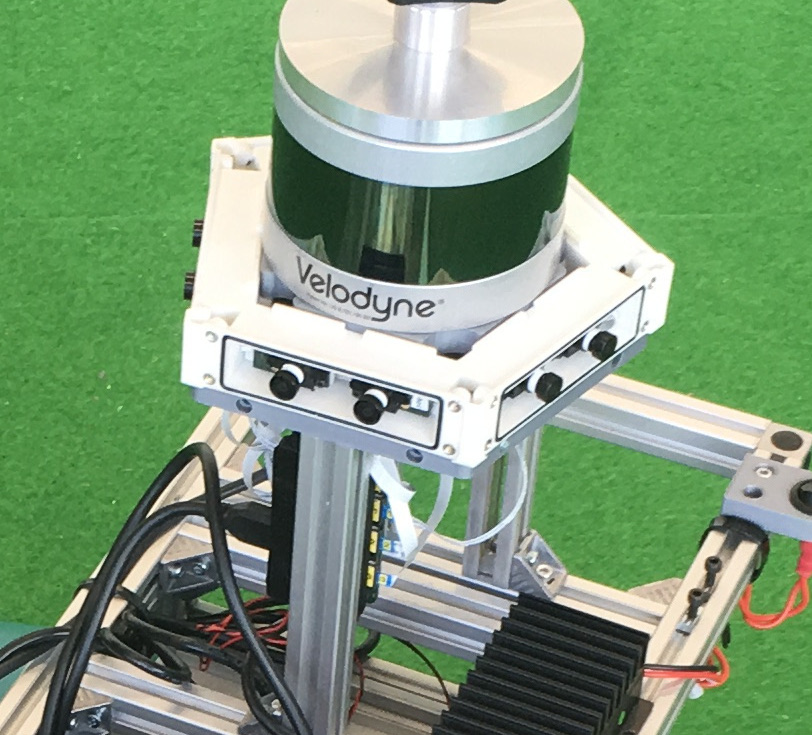
\includegraphics[width=0.4\textwidth]{cam_integration}\hspace{5mm}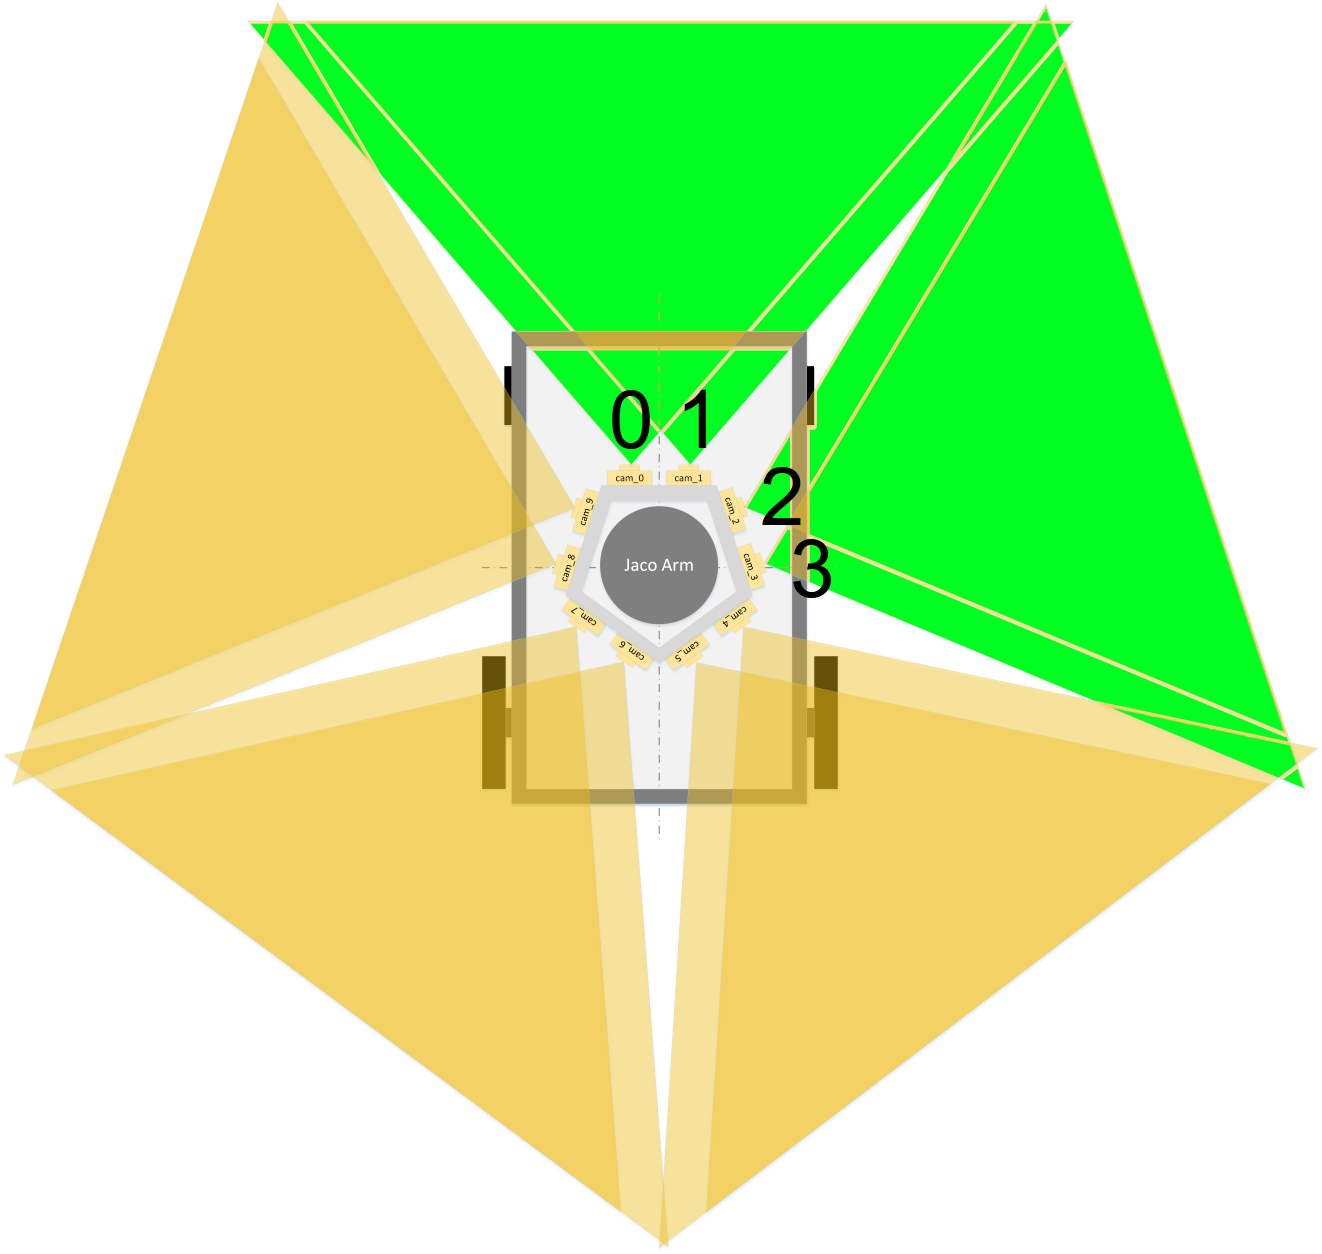
\includegraphics[width=0.4\textwidth]{cam_setup_3}
\end{frame}
%
\begin{frame}{Garden Dataset: Semantics and Depth}

\begin{columns}

\column{6cm}
\begin{itemize}
\item Set of 9 classes we distinguish
\begin{itemize}
\item Grass (light green)
\item Ground (brown)
\item Pavement (grey)
\item Hedge (ochre) 
\item Topiary (cyan)
\item Rose (red)
\item Obstacle (blue) 
\item Tree (dark green) 
\item Background (black)
\end{itemize}
\item Depth map from projected points
\end{itemize}

\column{5cm}

\includegraphics[width=1\columnwidth,bb = 0 0 200 100, draft, type=eps]{/home/radim/Documents/proj/TrimBot/Challenge2018/training/overcast_0001/vcam_0/vcam_0_f00001_over.png}

\includegraphics[width=1\columnwidth,bb = 0 0 200 100, draft, type=eps]{/home/radim/Documents/proj/TrimBot/Challenge2018/training/overcast_0001/vcam_0/vcam_0_f00001_dmap.png}
\end{columns}

\end{frame}
%
\begin{frame}{Garden Dataset: Training Point Clouds}

\begin{tabular}{cc}
\includegraphics[clip,width=0.4\textwidth,bb = 0 0 200 100, draft, type=eps]{/home/radim/Documents/proj/TrimBot/Challenge2018/gt/model_10mm_0001_rgb.png} & \includegraphics[clip,width=0.4\textwidth,bb = 0 0 200 100, draft, type=eps]{/home/radim/Documents/proj/TrimBot/Challenge2018/gt/model_10mm_0128_rgb.png}\tabularnewline
\includegraphics[clip,width=0.4\textwidth,bb = 0 0 200 100, draft, type=eps]{/home/radim/Documents/proj/TrimBot/Challenge2018/gt/model_10mm_0160_rgb.png} & \includegraphics[clip,width=0.4\textwidth,bb = 0 0 200 100, draft, type=eps]{/home/radim/Documents/proj/TrimBot/Challenge2018/gt/model_10mm_0224_rgb.png}\tabularnewline
\end{tabular}

\emph{Dataset rendered by Hoang-An Le (UvA)}
\end{frame}
%
\begin{frame}{Garden Dataset: Training Point Clouds}

\begin{tabular}{cc}
\includegraphics[clip,width=0.4\textwidth,bb = 0 0 200 100, draft, type=eps]{/home/radim/Documents/proj/TrimBot/Challenge2018/gt/model_10mm_0001_sem.png} & \includegraphics[clip,width=0.4\textwidth,bb = 0 0 200 100, draft, type=eps]{/home/radim/Documents/proj/TrimBot/Challenge2018/gt/model_10mm_0128_sem.png}\tabularnewline
\includegraphics[clip,width=0.4\textwidth,bb = 0 0 200 100, draft, type=eps]{/home/radim/Documents/proj/TrimBot/Challenge2018/gt/model_10mm_0160_sem.png} & \includegraphics[clip,width=0.4\textwidth,bb = 0 0 200 100, draft, type=eps]{/home/radim/Documents/proj/TrimBot/Challenge2018/gt/model_10mm_0224_sem.png}\tabularnewline
\end{tabular}

\emph{Dataset rendered by Hoang-An Le (UvA)}
\end{frame}
%
\begin{frame}{Garden Dataset: Test Point Cloud}

\includegraphics[width=1\textwidth,bb = 0 0 200 100, draft, type=eps]{/home/radim/Documents/proj/TrimBot/Challenge2018/gt/model_10mm_0288.png}

\emph{Dataset rendered by Hoang-An Le (UvA)}
\end{frame}
%
\begin{frame}{Garden Dataset: Validation Point Cloud}

\includegraphics[width=1\textwidth,bb = 0 0 200 100, draft, type=eps]{/home/radim/Documents/proj/TrimBot/Challenge2018/gt/model_10mm_real.png}
\end{frame}

\section{Evaluation and Results}
\begin{frame}{Submissions vs. Ground Truth}

\begin{tabular}{cc}
\includegraphics[clip,width=0.5\textwidth,bb = 0 0 200 100, draft, type=eps]{/home/radim/Documents/proj/TrimBot/Challenge2018/results/dtis/dtis_0288.png} & \includegraphics[clip,width=0.5\textwidth,bb = 0 0 200 100, draft, type=eps]{/home/radim/Documents/proj/TrimBot/Challenge2018/gt/model_10mm_0288.png}\tabularnewline
DTIS & GT\tabularnewline
\end{tabular}
\end{frame}
%
\begin{frame}{Submissions vs. Ground Truth}

\begin{tabular}{cc}
\includegraphics[clip,width=0.5\textwidth,bb = 0 0 200 100, draft, type=eps]{/home/radim/Documents/proj/TrimBot/Challenge2018/results/HAB/HAB_0288.png} & \includegraphics[clip,width=0.5\textwidth,bb = 0 0 200 100, draft, type=eps]{/home/radim/Documents/proj/TrimBot/Challenge2018/gt/model_10mm_0288.png}\tabularnewline
HAB & GT\tabularnewline
\end{tabular}
\end{frame}
%
\begin{frame}{Submissions vs. Ground Truth}

\begin{tabular}{cc}
\includegraphics[clip,width=0.5\textwidth,bb = 0 0 200 100, draft, type=eps]{/home/radim/Documents/proj/TrimBot/Challenge2018/results/lapsi360/lapsi360_0288.png} & \includegraphics[clip,width=0.5\textwidth,bb = 0 0 200 100, draft, type=eps]{/home/radim/Documents/proj/TrimBot/Challenge2018/gt/model_10mm_0288.png}\tabularnewline
LAPSI & GT\tabularnewline
\end{tabular}
\end{frame}
%
\begin{frame}{Evaluation Methodology}

\begin{itemize}
\item Test GT 
\begin{itemize}
\item delimited by the bounding box of the test area 
\end{itemize}
\item 3D geometry
\begin{itemize}
\item Submissions cropped to bounding box +1 m
\item Cumulative histograms of distances (mesh $\rightleftarrows$ GT points)
\item \textbf{Accuracy} is distance $d$ (in m) such that 90\% of the reconstruction
is within $d$ of the ground truth mesh
\item \textbf{Completeness} is the percent of points in the GT point cloud
that are within 5 cm of the reconstruction
\end{itemize}
\item Semantics
\begin{itemize}
\item Labels assigned to vertices or faces of the 3D model
\item Projected to all test images 
\item \textbf{Prediction accuracy} of the pixels corresponding to the 3D
test part
\end{itemize}
\end{itemize}
\end{frame}
%
\begin{frame}{Evaluation: 3D Geometry}

\begin{tabular}{cccc}
\includegraphics[clip,width=0.3\textwidth,bb = 0 0 200 100, draft, type=eps]{/home/radim/Documents/proj/TrimBot/Challenge2018/results/dtis/dtis_0288-acc.png} & \includegraphics[clip,width=0.3\textwidth,bb = 0 0 200 100, draft, type=eps]{/home/radim/Documents/proj/TrimBot/Challenge2018/results/HAB/HAB_0288-acc.png} & \includegraphics[clip,width=0.3\textwidth,bb = 0 0 200 100, draft, type=eps]{/home/radim/Documents/proj/TrimBot/Challenge2018/results/colmap/colmap_0288-acc.png} & \begin{turn}{90}
Accuracy
\end{turn}\tabularnewline
DTIS & HAB & COLMAP\footnote{\tiny Sch�nberger et al.: Structure-from-motion revisited. CVPR,
2016. } (baseline) & \tabularnewline
\includegraphics[clip,width=0.3\textwidth,bb = 0 0 200 100, draft, type=eps]{/home/radim/Documents/proj/TrimBot/Challenge2018/results/dtis/dtis_0288-comp.png} & \includegraphics[clip,width=0.3\textwidth,bb = 0 0 200 100, draft, type=eps]{/home/radim/Documents/proj/TrimBot/Challenge2018/results/HAB/HAB_0288-comp.png} & \includegraphics[clip,width=0.3\textwidth,bb = 0 0 200 100, draft, type=eps]{/home/radim/Documents/proj/TrimBot/Challenge2018/results/colmap/colmap_0288-comp.png} & \begin{turn}{90}
Completeness
\end{turn}\tabularnewline
\end{tabular}
\begin{itemize}
\item Distances {[}0-1m{]}: Cold colors indicate well reconstructed segments
\item Hot colors indicate noisy surface (accuracy) or missing parts (completeness).
\end{itemize}
\end{frame}
%
\begin{frame}{Evaluation: 3D Geometry (synthetic data)}
\begin{center}
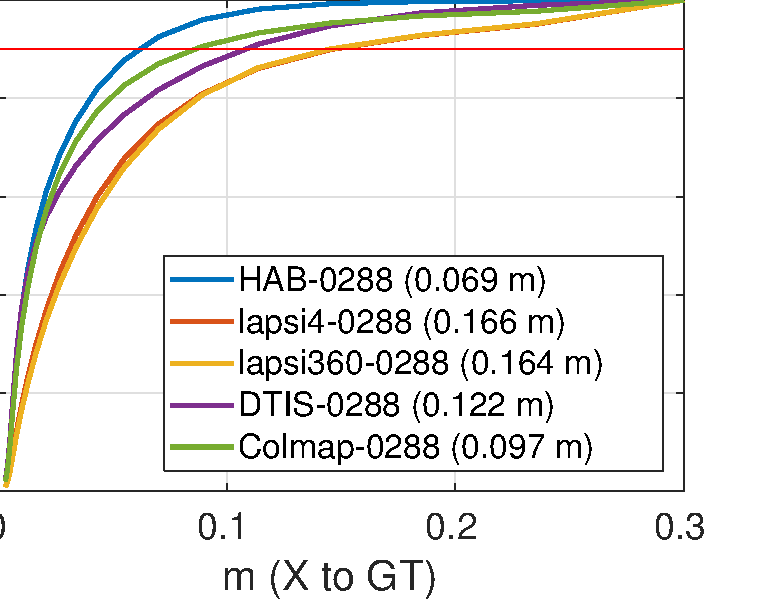
\includegraphics[clip,width=0.45\textwidth,bb = 0 0 200 100, draft, type=eps]{/home/radim/Documents/proj/TrimBot/Challenge2018/results/test-stats-acc.pdf}\hspace{5mm}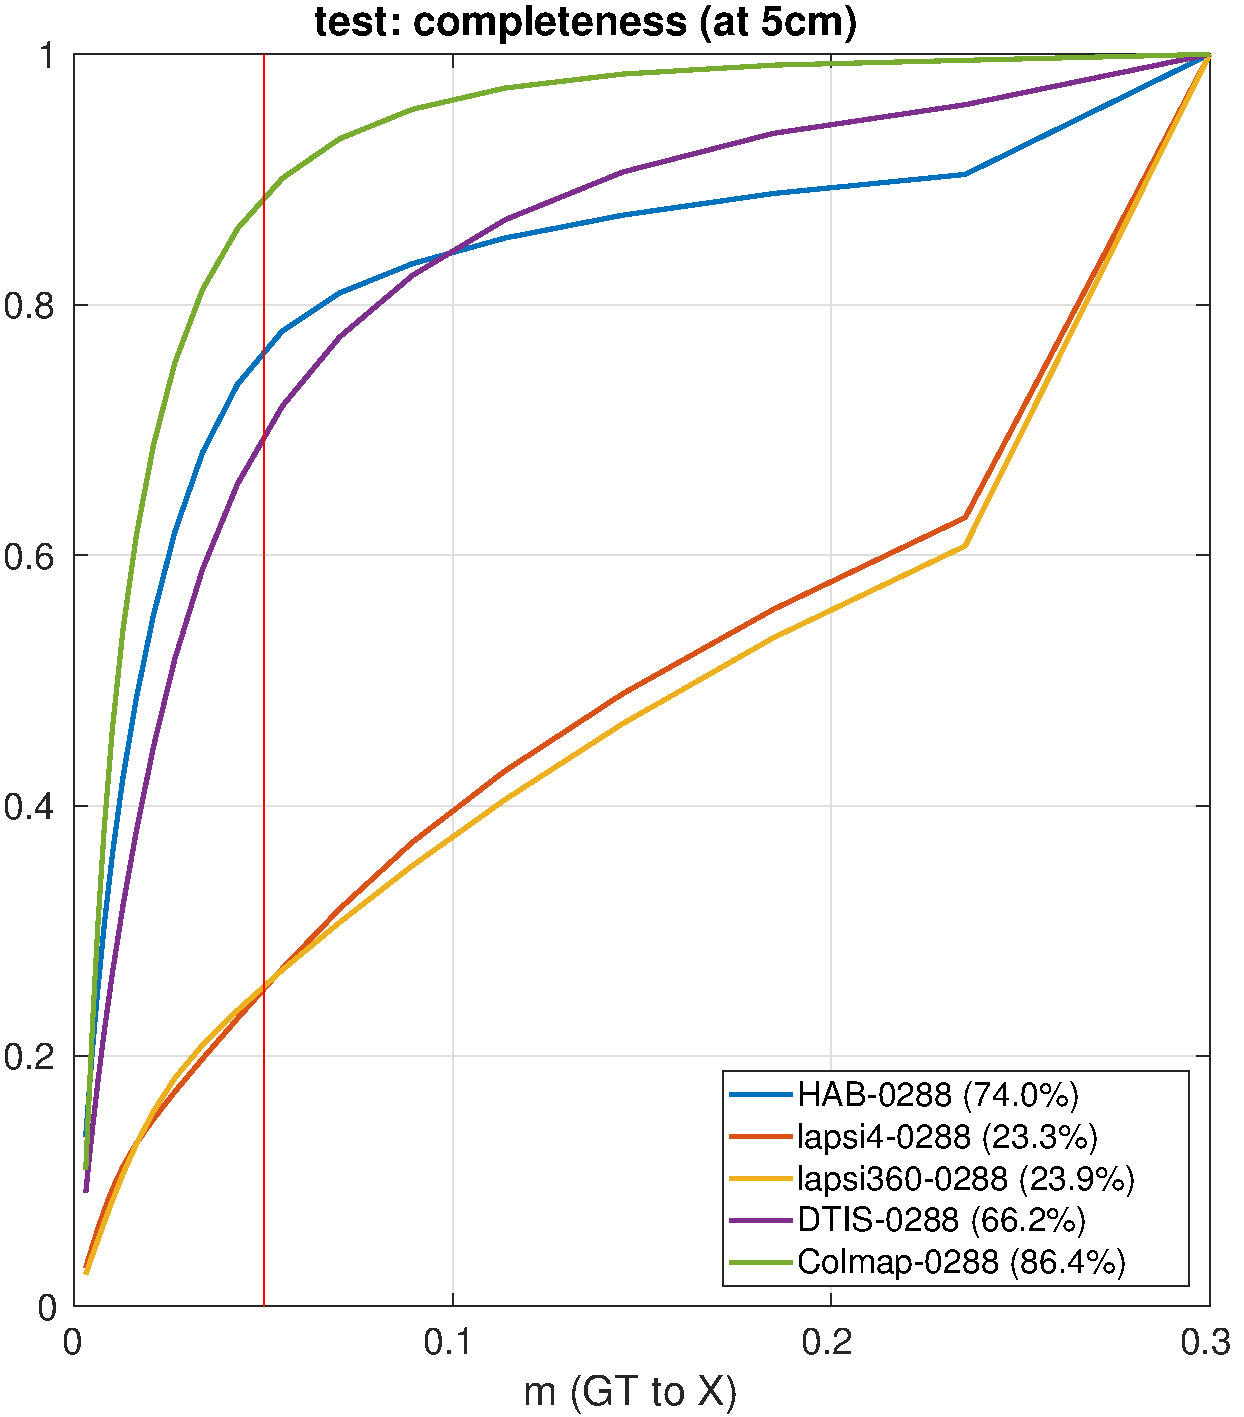
\includegraphics[clip,width=0.45\textwidth,bb = 0 0 200 100, draft, type=eps]{/home/radim/Documents/proj/TrimBot/Challenge2018/results/test-stats-comp.pdf}
\par\end{center}
\begin{itemize}
\item Cumulative plots of distances (mesh $\rightleftarrows$ GT points)
\end{itemize}
\end{frame}
%
\begin{frame}{Evaluation: 3D Geometry (real data)}
\begin{center}
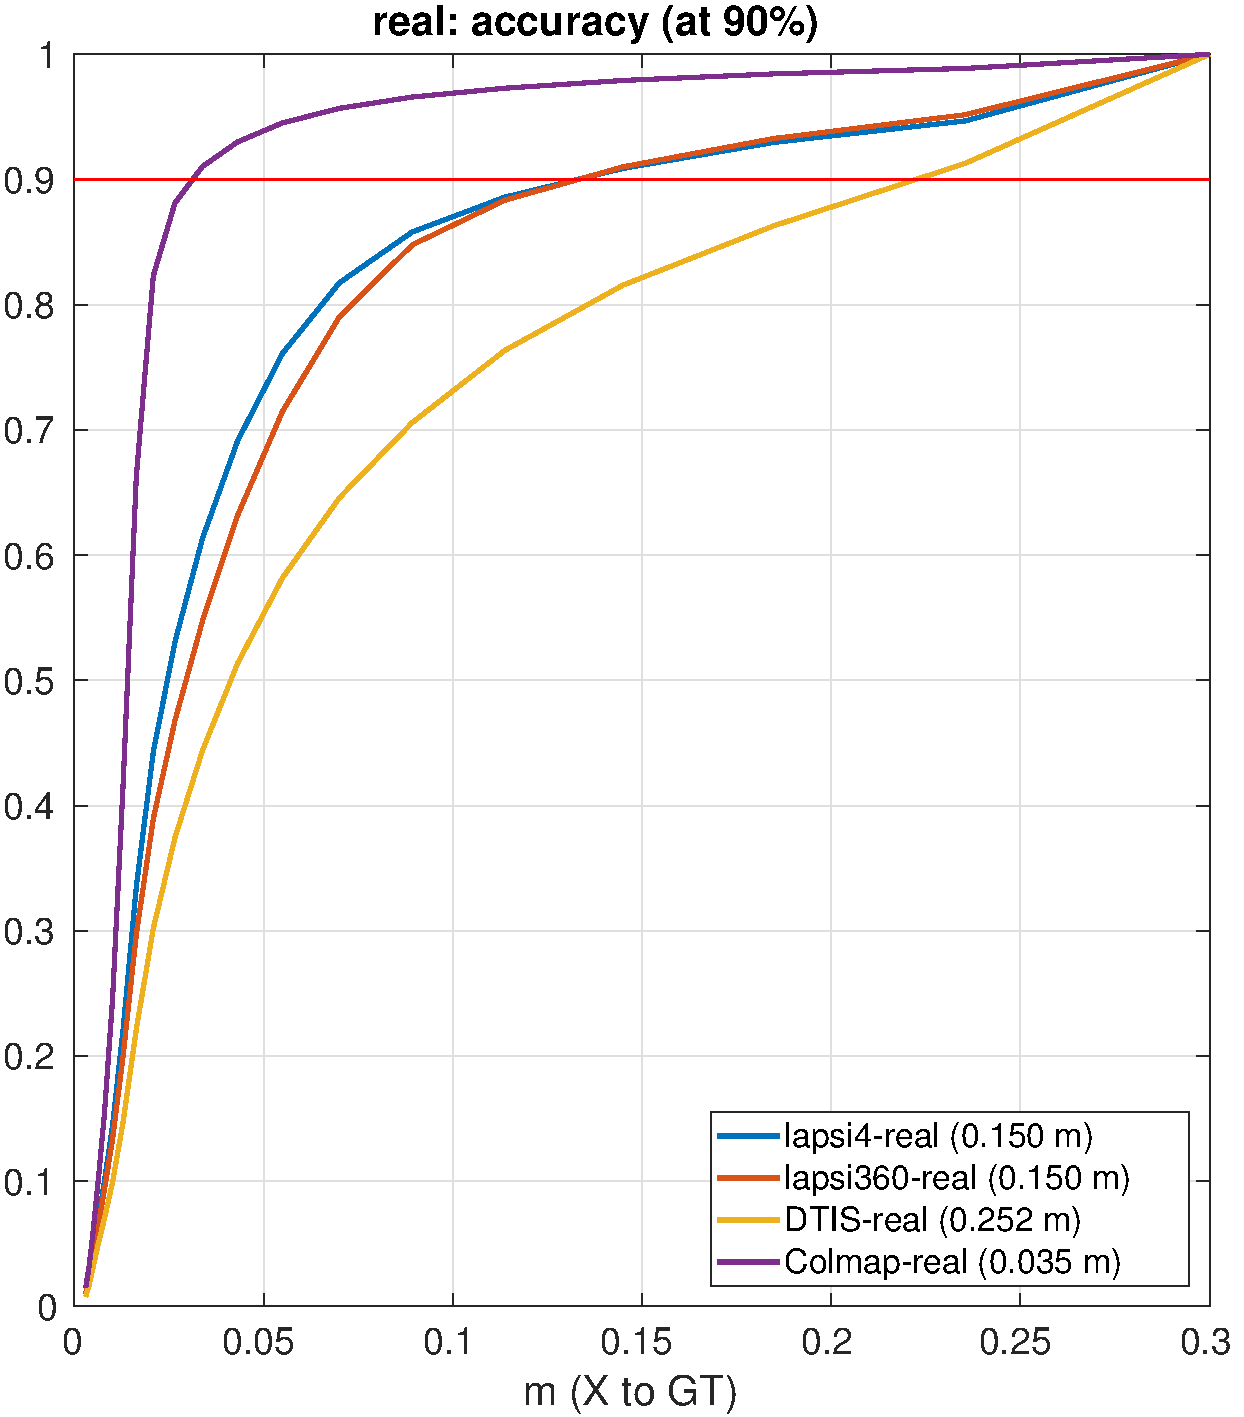
\includegraphics[clip,width=0.45\textwidth,bb = 0 0 200 100, draft, type=eps]{/home/radim/Documents/proj/TrimBot/Challenge2018/results/real-stats-acc.pdf}\hspace{5mm}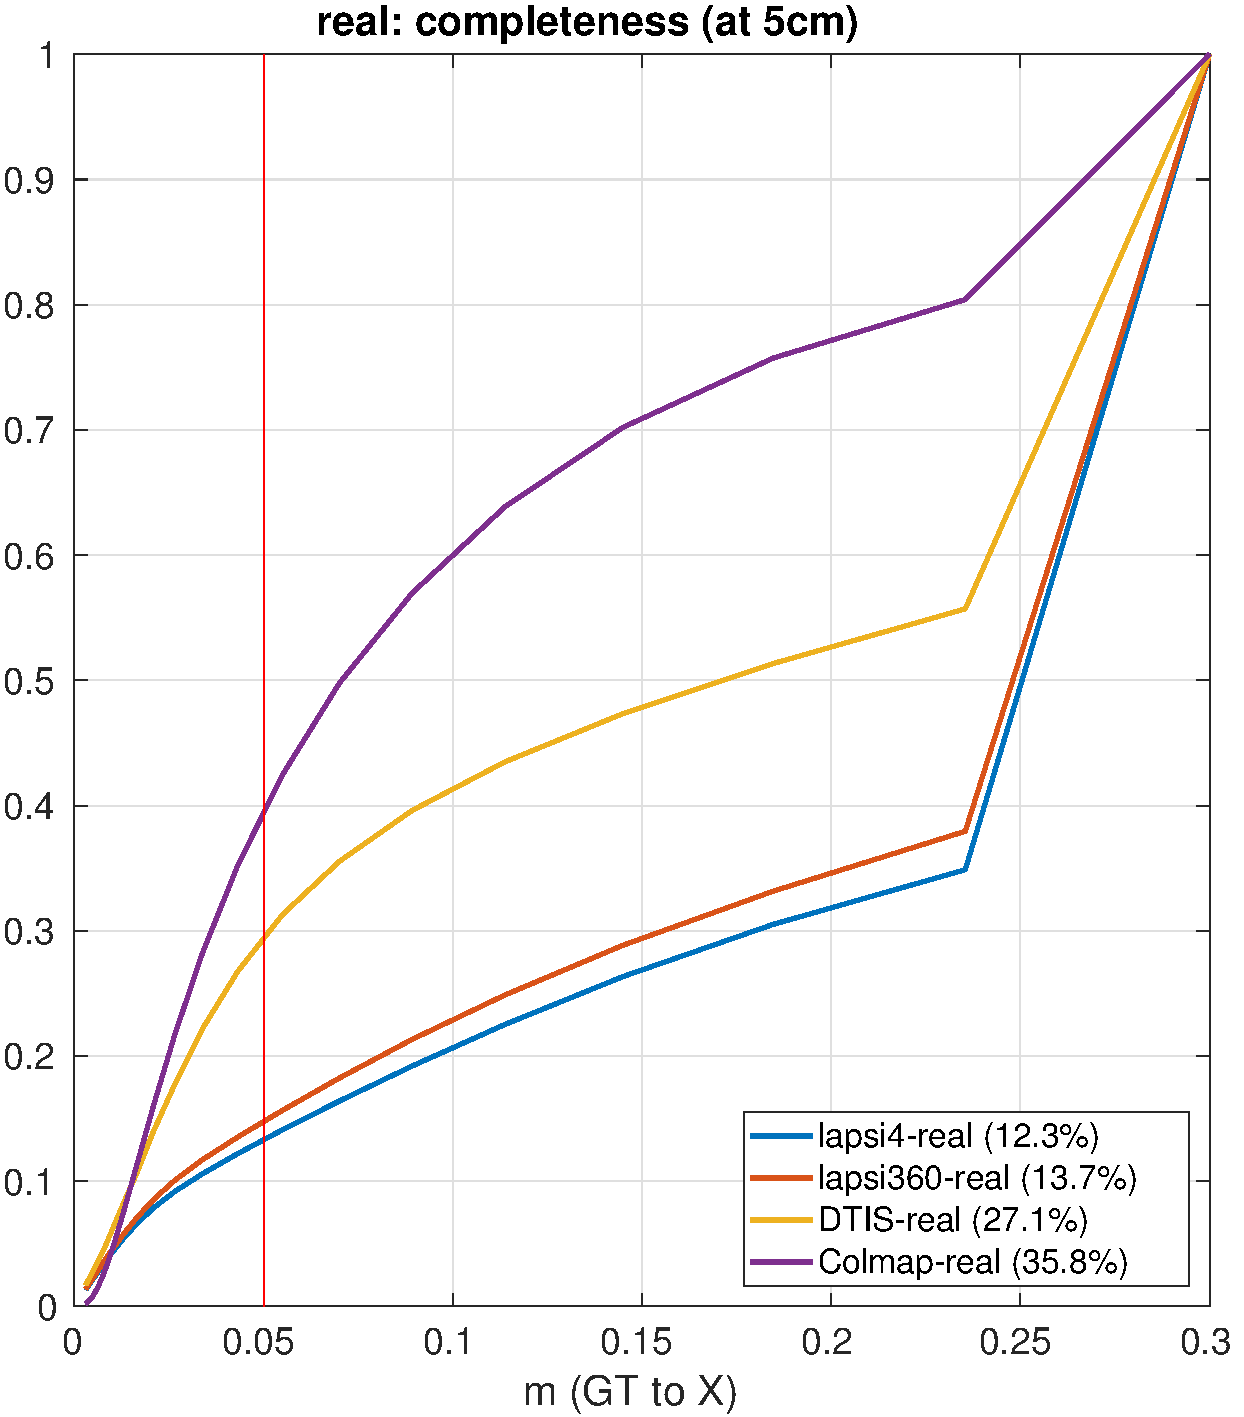
\includegraphics[clip,width=0.45\textwidth,bb = 0 0 200 100, draft, type=eps]{/home/radim/Documents/proj/TrimBot/Challenge2018/results/real-stats-comp.pdf}
\par\end{center}
\begin{itemize}
\item Cumulative plots of distances (mesh $\rightleftarrows$ GT points)
\end{itemize}
\end{frame}
%
\begin{frame}{Evaluation: Semantics (synthetic data)}

\begin{tabular}{cccc}
\includegraphics[clip,width=0.3\textwidth,bb = 0 0 200 100, draft, type=eps]{/home/radim/Documents/proj/TrimBot/Challenge2018/results/dtis/clear_0288/vcam_0/vcam_0_f00001_undist.png} & \includegraphics[clip,width=0.3\textwidth,bb = 0 0 200 100, draft, type=eps]{/home/radim/Documents/proj/TrimBot/Challenge2018/results/HAB/clear_0288/vcam_0/vcam_0_f00001_undist.png} & \includegraphics[clip,width=0.3\textwidth,bb = 0 0 200 100, draft, type=eps]{/home/radim/Documents/proj/TrimBot/Challenge2018/results/snfull-frImgNet/clear_0288/vcam_0/vcam_0_f00001_undist_flip.png} & \begin{turn}{90}
Prediction
\end{turn}\tabularnewline
DTIS & HAB & SegNet\footnote{\tiny Badrinarayanan et al.: SegNet: A deep convolutional encoder-decoder
architecture for image segmentation. PAMI, 2017.} (baseline) & \tabularnewline
\includegraphics[clip,width=0.3\textwidth,bb = 0 0 200 100, draft, type=eps]{/home/radim/Documents/proj/TrimBot/Challenge2018/results/dtis/clear_0288/vcam_0/vcam_0_f00001_err.png} & \includegraphics[clip,width=0.3\textwidth,bb = 0 0 200 100, draft, type=eps]{/home/radim/Documents/proj/TrimBot/Challenge2018/results/HAB/clear_0288/vcam_0/vcam_0_f00001_err.png} & \includegraphics[clip,width=0.3\textwidth,bb = 0 0 200 100, draft, type=eps]{/home/radim/Documents/proj/TrimBot/Challenge2018/results/snfull-frImgNet/clear_0288/vcam_0/vcam_0_f00001_err.png} & \begin{turn}{90}
Error mask
\end{turn}\tabularnewline
\end{tabular}
\begin{itemize}
\item Error: \emph{red} incorrect pixels, \emph{grey} correct, \emph{black}
not evaluated
\item SegNet: pre-trained with ImageNet + challenge training set
\end{itemize}
\end{frame}
%
\begin{frame}{Evaluation: Semantics (synthetic data)}

\begin{tabular}{cccc}
\includegraphics[clip,width=0.3\textwidth,bb = 0 0 200 100, draft, type=eps]{/home/radim/Documents/proj/TrimBot/Challenge2018/gt/clear_0288/vcam_0/vcam_0_f00001_gtr.png} & \includegraphics[clip,width=0.3\textwidth,bb = 0 0 200 100, draft, type=eps]{/home/radim/Documents/proj/TrimBot/Challenge2018/gt/clear_0288/vcam_0/vcam_0_f00001_gtr.png} & \includegraphics[clip,width=0.3\textwidth,bb = 0 0 200 100, draft, type=eps]{/home/radim/Documents/proj/TrimBot/Challenge2018/gt/clear_0288/vcam_0/vcam_0_f00001_gtr.png} & \begin{turn}{90}
GT
\end{turn}\tabularnewline
DTIS & HAB & SegNet\footnote{\tiny Badrinarayanan et al.: SegNet: A deep convolutional encoder-decoder
architecture for image segmentation. PAMI, 2017.} (baseline) & \tabularnewline
\includegraphics[clip,width=0.3\textwidth,bb = 0 0 200 100, draft, type=eps]{/home/radim/Documents/proj/TrimBot/Challenge2018/results/dtis/clear_0288/vcam_0/vcam_0_f00001_err.png} & \includegraphics[clip,width=0.3\textwidth,bb = 0 0 200 100, draft, type=eps]{/home/radim/Documents/proj/TrimBot/Challenge2018/results/HAB/clear_0288/vcam_0/vcam_0_f00001_err.png} & \includegraphics[clip,width=0.3\textwidth,bb = 0 0 200 100, draft, type=eps]{/home/radim/Documents/proj/TrimBot/Challenge2018/results/snfull-frImgNet/clear_0288/vcam_0/vcam_0_f00001_err.png} & \begin{turn}{90}
Error mask
\end{turn}\tabularnewline
\end{tabular}
\begin{itemize}
\item Error: \emph{red} incorrect pixels, \emph{grey} correct, \emph{black}
not evaluated
\item SegNet: pre-trained with ImageNet + challenge training set
\end{itemize}
\end{frame}
%
\begin{frame}{Evaluation: Semantics (synthetic data)}

\begin{tabular}{ccc}
\includegraphics[clip,width=0.3\textwidth,bb = 0 0 200 100, draft, type=eps]{/home/radim/Documents/proj/TrimBot/Challenge2018/results/dtis/test-sem-all-conf.pdf} & \includegraphics[clip,width=0.3\textwidth,bb = 0 0 200 100, draft, type=eps]{/home/radim/Documents/proj/TrimBot/Challenge2018/results/HAB/test-sem-all-conf.pdf} & \includegraphics[clip,width=0.3\textwidth,bb = 0 0 200 100, draft, type=eps]{/home/radim/Documents/proj/TrimBot/Challenge2018/results/snfull-frImgNet/test-sem-all-conf.pdf}\tabularnewline
\textbf{91.1\%} & 79.0\% & 90.2\%\tabularnewline
DTIS & HAB & SegNet (baseline)\tabularnewline
\end{tabular}
\begin{itemize}
\item Confusion matrix: \emph{dark }on diagonal indicates good match of
the prediction with GT labels
\item Semantic accuracy: pixelwise ratio of correct predictions over all
test images
\end{itemize}
\end{frame}
%
\begin{frame}{Evaluation: Summary of Performance}
\begin{center}
\begin{tabular}{|c|c|c|c|}
\hline 
\multirow{2}{*}{\emph{Method}} & \multicolumn{2}{c|}{3D Reconstruction} & \emph{Semantic}\tabularnewline
\cline{2-4} 
 & \emph{Accuracy} & \emph{Completeness} & \emph{Accuracy}\tabularnewline
\hline 
\hline 
DTIS & 0.122 m & 66.2 \% & \textbf{91.1 \%}\tabularnewline
\hline 
HAB & \textbf{0.069 m} & \textbf{74.0 \%} & 79.0 \%\tabularnewline
\hline 
LAPSI & 0.164 m & 23.9 \% & \tabularnewline
\hline 
Baseline & \emph{0.097 m} & \emph{86.4 \%} & \emph{90.2 \%}\tabularnewline
\hline 
\end{tabular}
\par\end{center}

\begin{center}
Test set (Synthetic data)
\par\end{center}

\end{frame}
%
\begin{frame}{Evaluation: Summary of Performance}
\begin{center}
\begin{tabular}{|c|c|c|c|}
\hline 
\multirow{2}{*}{\emph{Method}} & \multicolumn{2}{c|}{3D Reconstruction} & \emph{Semantic}\tabularnewline
\cline{2-4} 
 & \emph{Accuracy} & \emph{Completeness} & \emph{Accuracy}\tabularnewline
\hline 
\hline 
DTIS & 0.25 m & \textbf{27.1 \%} & \textbf{65.7 \%}\tabularnewline
\hline 
HAB &  &  & \tabularnewline
\hline 
LAPSI & \textbf{0.15 m} & 13.7 \% & \tabularnewline
\hline 
Baseline & \emph{0.035 m} & \emph{35.8 \%} & \emph{85.4 \%}\tabularnewline
\hline 
\end{tabular}
\par\end{center}

\begin{center}
Validation set (Real data)
\par\end{center}

\end{frame}
%
\begin{frame}{Challenge Results Summary}
\begin{itemize}
\item Best performers for \textbf{synthetic} data
\begin{itemize}
\item Semantic category: DTIS
\item 3D Geometry category: HAB
\end{itemize}
\item Best performer for \textbf{real} data: DTIS
\end{itemize}
\medskip{}
\rule[0.5ex]{1\columnwidth}{1pt}

\textbf{}%
\begin{tabular}{>{\centering}p{1\textwidth}}
\textbf{Congratulations and thanks to all participants!}\tabularnewline
We are open to additional submissions.\tabularnewline
\end{tabular}

\end{frame}

\end{document}
